\documentclass{beamer}
\mode<presentation>
\setbeamertemplate{bibliography item}{}
\usepackage[utf8]{vietnam}
\usepackage{beamerthemesplit}
\usepackage{graphicx}
\usepackage{booktabs}
\usepackage{amsmath}
\usepackage{textpos}
\usepackage{pgfplots}
\usepackage{tikz}
\usepackage{hyperref}
\usepackage{caption}
\usetikzlibrary{shapes.geometric, arrows}
\usetikzlibrary {datavisualization} 
\pgfplotsset{compat=1.18, width = 7cm}
\usetikzlibrary{patterns}
\setbeamertemplate{bibliography item}[text]
%\usepackage{customTheme} % Include the custom theme
%\usepackage{hsmr} % Include the custom theme
\usetheme{Ilmenau} % AnnArbor, Ilmenau, Darmstadt, Dresden, CambridgeUS, Frankfurt, Singapore
\newtheorem{dn}{Định nghĩa}[section]
\newtheorem{dl}{Định lý}[section]
\newtheorem{tc}{Tính chất}[section]
\newtheorem{hq}{Hệ quả}[section]
\newtheorem{bd}{Bổ đề}[section]
\newtheorem{md}{Mệnh đề}[section]
\newtheorem{vd}{Ví dụ}[section]
\newtheorem{nx}{Nhận xét}[section]
\newcommand{\dom}{\text{{\rm dom}}}
\newcommand{\epi}{\text{{\rm epi}}}
\newcommand{\Min}{\text{{\rm Min}}}
\setbeamertemplate{theorems}[numbered]
\setbeamertemplate{definitions}[numbered]
\setbeamertemplate{footline}[frame number]
\usepackage{algorithm}
\usepackage{color}
\usepackage{algorithmic}
\usepackage{footmisc}
\usepackage{indentfirst} 
\usepackage{comment}
\AtBeginEnvironment{proof}{%
  \setbeamercolor{block title}{use=example text,fg=white,bg=example text.fg!75!black}
  \setbeamercolor{block body}{parent=normal text,use=block title example,bg=block title example.bg!10!bg}
}
\renewcommand{\thefootnote}{\arabic{footnote}}
\usefonttheme{professionalfonts}
\setbeamercolor{normal text}{bg=white,fg=black}
\renewcommand{\thefootnote}{\arabic{footnote}}
\beamertemplatetransparentcoveredhigh
\begin{document}
\title[]{\fontsize{13pt}{10pt}\selectfont {\bf \LARGE   Phương pháp giải bài toán \\Tối ưu tuyến tính nguyên}\\
------------------------------------------

{\small Hướng dẫn: PGS.TS. Tạ Quang Sơn}} 
\author[]{\bf Thực hiện : ĐỖ NGỌC MINH THƯ \& NGUYỄN CHÍ BẰNG \\
Sinh viên lớp: DTU1221, Khóa: 22}
\institute[Báo cáo luận văn thạc sĩ]{\fontsize{2pt}{2pt}}%
\small{\date{\today}}
\begin{frame}
\begin{center}
{\fontsize{8pt}{8pt}\selectfont \bf{ỦY BAN NHÂN DÂN THÀNH PHỐ HỒ CHÍ MINH\\
TRƯỜNG ĐẠI HỌC SÀI GÒN}}
\end{center}
\begin{center}
\end{center}

\begin{center}
{\fontsize{10pt}{6pt}\selectfont \bf{BÁO CÁO ĐỀ CƯƠNG NGHIÊN CỨU KHOA HỌC\\
NGÀNH: TOÁN ỨNG DỤNG}}
\end{center}
\titlepage
\end{frame}
\begin{frame}
    \frametitle{NỘI DUNG BÁO CÁO}
    \tableofcontents
\end{frame}

% Tai sao quan tam de tai?
% Lam duoc gi?
% Hoc duoc gi ?
% Du dinh tiep theo ?
% - - -
% Cơ sở lý thuyết và Mục tiêu
\section{Giới thiệu}

\begin{frame}
   \center 
   \huge Giới thiệu
\end{frame}


\begin{frame}{\bf Mục đích nghiên cứu}
\textbf{Tối ưu tuyến tính} là một nội dung quan trọng trong chương trình đào tạo Cử nhân Toán ứng dụng. Lý thuyết về việc giải bài toán tối ưu tuyến tính đã được cung cấp cho sinh viên. Tuy vậy, có nhiều bài toán tối ưu cần được giải với nghiệm nguyên. Chẳng hạn như:
\begin{itemize}
\item Bài toán tối ưu nhân lực.
\item Bài toán tối ưu vận chuyển hàng hóa.
\item Bài toán tối ưu áp dụng trong tin học.
\end{itemize}

\bigskip
Có một lý thuyết riêng cho việc xử lý các bài toán Tối ưu tuyến tính và \textcolor{red}{tìm nghiệm nguyên.}
\bigskip

{\it Mục đích của đề tài này là tìm hiểu một số phương pháp giải bài toán Tối ưu tuyến tính và tìm nghiệm nguyên cho bài toán.}  
\end{frame}

\begin{frame}{\bf Tại sao cần có một lý thuyết riêng cho bài toán Tối ưu tuyến tính nguyên}

\begin{columns}
    \begin{column}{0.5\textwidth}
        \begin{equation*}
        \begin{array}{lll}            
        {\rm Max}&f(x)=2x_1+2x_2\\
        & \begin{cases}
        2x_1+x_2 \leq  8 \\
        x_1+3x_2 \leq 10 \\
        x_i\geq 0,\forall i=1,2.
        \end{cases} 
        \end{array}
        \end{equation*}
    \end{column}

    \begin{column}{0.5\textwidth}
        \begin{figure}
        \centering
        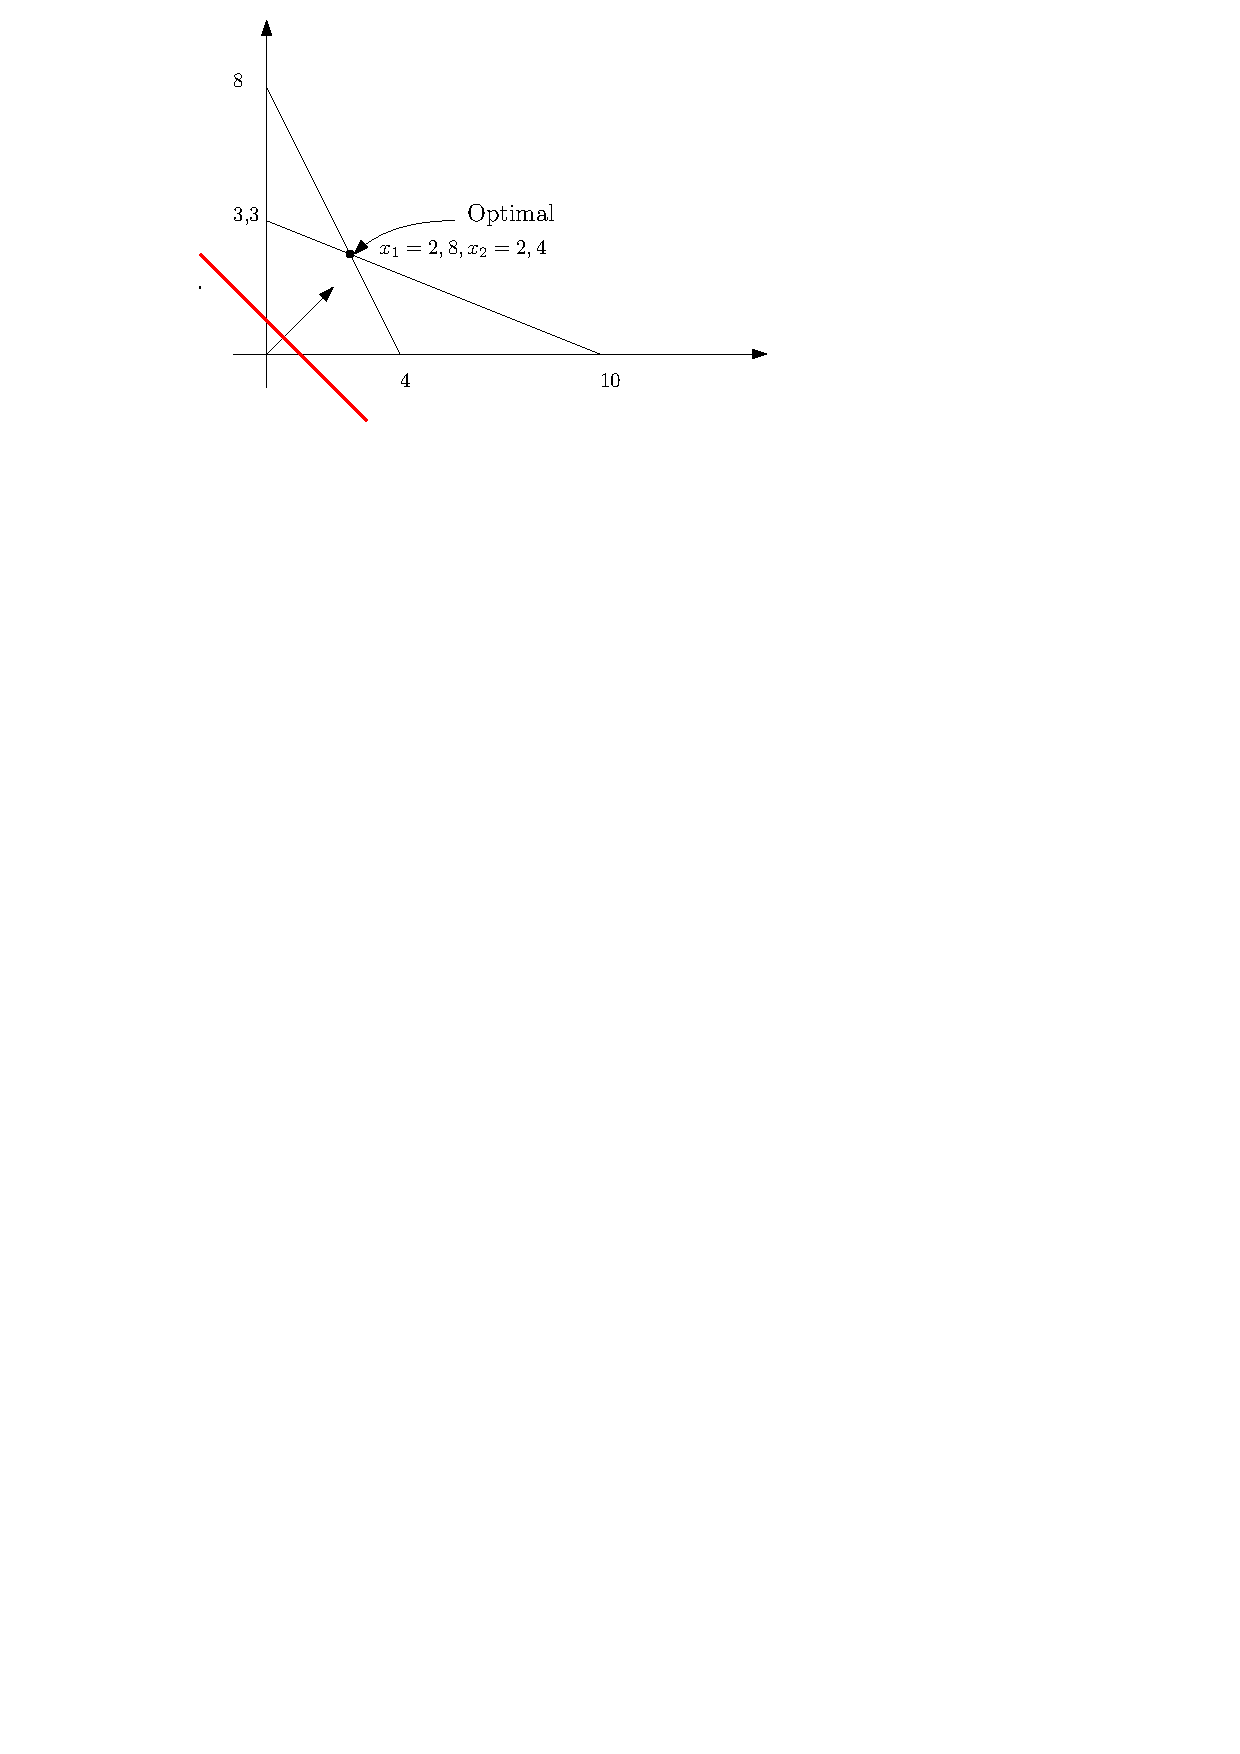
\includegraphics[width=1\linewidth]{Nhom1_hinh.pdf}
        \caption{Hình minh hoạ bài toán}
        \end{figure}
    \end{column}
\end{columns}
\end{frame}


\begin{frame}{\bf Nhận xét}

$\bullet$  Nếu giải bài toán trên bằng phương pháp thông thường, ta nhận được nghiệm $x_1=2.8$, $x_2=2.4$.
\medskip
      
      $\bullet$ Nếu làm tròn nghiệm $x_1 \to 3$ và $x_2 \to 3$ thì điểm $(x_1,x_2)$ không còn thuộc miền chấp nhận được.
      
 \medskip
      
      $\bullet$ Nếu làm tròn nghiệm $x_1 \to 2$ và $x_2 \to 2$ thì điểm $(x_1,x_2)$ chưa biết có phải nghiệm tối ưu hay không?
      
\bigskip
 \textcolor{red}{\bf Nếu giải bài toán QHTT rồi sau đó làm tròn số thì có thể  cho kết không như mong đợi.}
   
\end{frame}

\section{Phương pháp lát cắt Gomory}
\begin{frame}
   \center 
   \huge Phương pháp lát cắt Gomory
\end{frame}





\section{Phương pháp Land-Doig (Nhánh cận)}
\begin{frame}
    \center 
    \huge Phương pháp Land-Doig (Nhánh cận)
 \end{frame}





\section{Kết luận và Hướng phát triển}
\begin{frame}
    \center 
    \huge Kết luận
 \end{frame}

\begin{frame}
    \center 
    \huge Hướng phát triển
 \end{frame}
\section{Tài liệu tham khảo}

%sample
\begin{frame}
\end{frame}

\begin{frame}
    \begin{block}{}
    \medskip
    \center{\huge \it \textcolor[rgb]{0.50,0.30,1.0}{Cảm ơn quý thầy cô và các anh chị đã quan tâm theo dõi!}}
    \medskip
    \end{block}	
\end{frame}    
\end{document}